\documentclass[11pt]{article}
\usepackage[utf8]{inputenc}
\usepackage[ngerman]{babel}

\usepackage{amsmath,amsthm,amssymb,amsfonts}

\usepackage{graphicx}
\graphicspath{{abb/4-rotation-kin/}}
\usepackage{float}
\usepackage{tikz}

\usepackage{fancyhdr} % For headers and footers
\usepackage{geometry}
\usepackage{listings}
\usepackage{hyperref}
\hypersetup{
    linkcolor=blue,     
    urlcolor=cyan,
}

\geometry{
    a4paper, % Change this if you intend to print on a different paper size, such as letter paper.
    left=20mm,
    right=20mm,
    top=30mm,
    bottom=30mm,
}

\newcount\colveccount
\newcommand*\colvec[1]{
        \global\colveccount#1
        \begin{pmatrix}
        \colvecnext
}
\def\colvecnext#1{
        #1
        \global\advance\colveccount-1
        \ifnum\colveccount>0
                \\
                \expandafter\colvecnext
        \else
                \end{pmatrix}
        \fi
}

\title{Kinematik - Rotation}
\author{Emil Staikov}
\date{17. Mai 2021}

\begin{document}
\maketitle
Allgemeine Rotationen oder Drehungen kann man sich leicht vorstellen, die physikalische Modellierung wird aber stellenweise sehr komplex. Für uns reicht es aus, Drehungen in einer Ebene um eine fixierte Achse zu betrachten. Komplexere Bewegungen können wir tatsächlich aus der uns bereits bekannten Translationsbewegung und (teils mehreren) solchen einfachen Rotationen zusammensetzen. 

\section{Winkelgrößen}
\begin{figure}[H]
        \centering
        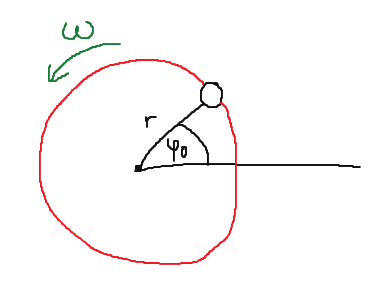
\includegraphics[width=0.5\textwidth]{rotation.png}
        \caption{Draufsicht für eine Rotationsbewegung in der Ebene, der schwarze Punkt in der Mitte symbolisiert die zur Seite senkrecht stehende Rotationsachse}
\end{figure}
Bei der Rotation bietet es sich an, die momentane Lage des Objekts durch den Abstand zur Rotationsachse $r$, sowie den Winkel $\varphi$ im Verhältnis zu einer fest gewählten Position zu beschreiben (s. Polarkoordinaten, bzw. Darstellung eines Vektors in Polarform). In $\varphi$ verhält sich die Rotationsbewegung praktisch wie die Translationsbewegung in $\vec{s}$, wir definieren entsprechend zur Translationsbewegung: 
\begin{itemize}
        \item Winkelgeschwindikeit $\displaystyle\omega = \frac{\Delta \varphi}{\Delta t}$
        \item Winkelbeschleunigung $\displaystyle\alpha = \frac{\Delta \omega}{\Delta t}$
\end{itemize}
Genau wie bei der Translationsbewegung können wir $\varphi(t)$ herleiten: 
\begin{itemize}
        \item $\omega = const.$ \\
                $\varphi(t) = \omega t + \varphi_0$
        \item $\alpha = const.$ \\
                $\omega(t) = \alpha t + \omega_0$ \\
                $\varphi(t) = \frac{1}{2}\alpha t^2 + \omega_0 t + \varphi_0$ 
\end{itemize}

\section{Lineare Größen}
Wir können auch die absolute Bogenlänge $s$ nutzen, um die Lage des rotierenden Objekts zu beschreiben. Wir können aus dem Winkel $\varphi$ im Bogenmaß stets die absolute Bogenlänge errechnen: 
\begin{align*}
        s = r\varphi
\end{align*}
Die Änderung der Bogenlänge ergibt sich dann zu 
\begin{align*}
        \frac{\Delta s}{\Delta t} = \frac{\Delta r\varphi}{\Delta t} = r \frac{\Delta \varphi}{\Delta t} = r\omega
\end{align*}
$\frac{\Delta t}{\Delta s}$ ist gleichzeitig die lineare Geschwindigkeit in tangentialer Richtung, also die sogenannte Tangentialgeschwindigkeit $v_T$. Also: 
\begin{align*}
        v_T = r\omega
\end{align*}
Die als Änderung der Tangentialgeschwindigkeit definierte Tangentialbeschleunigung $a_T$ ergibt sich dann zu: 
\begin{align*}
        a_t = \frac{\Delta v_T}{\Delta t} = \frac{\Delta r\omega}{\Delta t} = r \frac{\Delta \omega}{\Delta t} = r\alpha
\end{align*}
\end{document}
